% !TEX root = ../main.tex
\newpage
\section{Mean Field Reductions}
\subsection{The Ott-Antonsen manifold for fully connected networks}
In \cite{OttAntonsen2008, OttAntonsen2009, OttAntonsen2010} a method was published to predict the dynamics of the order parameter \eqref{eq:orderparameter} for a fully connected network ($A_{ij} = 1$) of oscillators. The authors explore a continuum interpretation of the mean field, in the limit that  $N \gg 1$. It is assumed that the state of of the neurons can be represented by a continuous probability distribution, $f(\theta, \eta \rvert \k, t)$, so that $g(\eta \rvert \k) = \int f \mathop{d\theta}$. The number of oscillators is constant, so that $f$ is constrained by a continuity equation, and it is shown that there exists a manifold of invariant probability densities to which the dynamics are attracted to. We are left with a simplified description of the dynamics of the network, the \textsl{mean-field reduction} (\MFR). The exact \MFR is obtained by expanding $g$ as a Fourier series, and expanding the pulse $\mathcal{P}_n$ using the binomial theorem. When assuming $\eta_i$ is distributed according to a Lorenz distribution:
\begin{align}
g(\eta | \k)=\frac{1}{\pi} \frac{\sigma(\k)}{(\eta-\eta_{0}(\k))^{2}+\sigma(\k)^{2}} \label{eq:Lorentzpdf}
\end{align}
the set of reduced equations then takes a particularly simple form, as the continuity equation can be evaluated at the poles of $g$ using the Cauchy residue theorem for the integration of complex variables and one find a closed form expression.


\subsection{Dynamics of the mean field}
Using this approach, the \MFR becomes \cite{Luke2013, Martens2020}:
\begin{align}
\dot{Z}(t)= -\ic \frac{(Z-1)^2}{2}+\frac{(Z+1)^2}{2} \cdot \left(-\sigma+ \ic\eta_{0}
+ \ic \kappa \cdot \left(1+\frac{Z^{2} + \overline{Z}^{2} }{6} - \frac{4}{3} \Re(Z)\right)\right) \label{eq:MeanField}
\end{align}
We can now describe the mean-field dynamics using \eqref{eq:MeanField}, and as it is a complex-valued function, the reduced system is two-dimensional, with three bifurcation parameters $\eta_0, \sigma$ and $\k$. For a fully connected network, three distinct macroscopic states can be identified.\\
In the partially synchronous rest state (\PSR) we can observe in Figure \ref{fig:MFRPSR}, $\bar{Z}(t)$ settles onto a stable node. Most neurons can be found in a resting state $\eta_0 + \sigma \lesssim 0$, and inhibit one another through $\kappa < 0$. Most neurons are therefore inactive, though some spiking neurons from the tail of $g(\eta)$ are present but have a neglegible effect. \\

In Figure \ref{fig:MFRPSS} we can observe a partially synchronous spiking (\PSS) state, where we can see how $\bar{Z}(t)$ settles onto a stable focus. This happens predominantly when $\eta_0 - \sigma \gtrsim 0$ and most neurons inherently spike, with the coupling being either excitatory or weakly inhibitory. Although most neurons are active, the network is partially synchronous and organized such that phase cancellation occurs by continuous spiking among the neurons.\\

Lastly, in the collective periodic wave state (\CPW) we can observe a limit cycle of the mean field, in Figure \ref{fig:MFRCPW}. Most neurons are active and inhibitory: $\eta_0 > 0$ and $k < 0$. The collective oscillation emerges from the interplay between the neurons’ inherent tendency to spike and the strong suppressive network interaction. \CPW states are mediated through Hopf bifurcations and homoclinic bifurcations of $Z(t)$. We can also see the occurrence of a saddle-node bifurcation in the lower hand corner, for low $\sigma$. We will continue to study the \CPW due to their interesting properties.\\
A more detailed discussion of the different regimes and bifurcations can be found in \cite{Luke2013}.

\begin{figure}[H]
\centering
\begin{subfigure}[b]{0.32\linewidth}
   \centering
  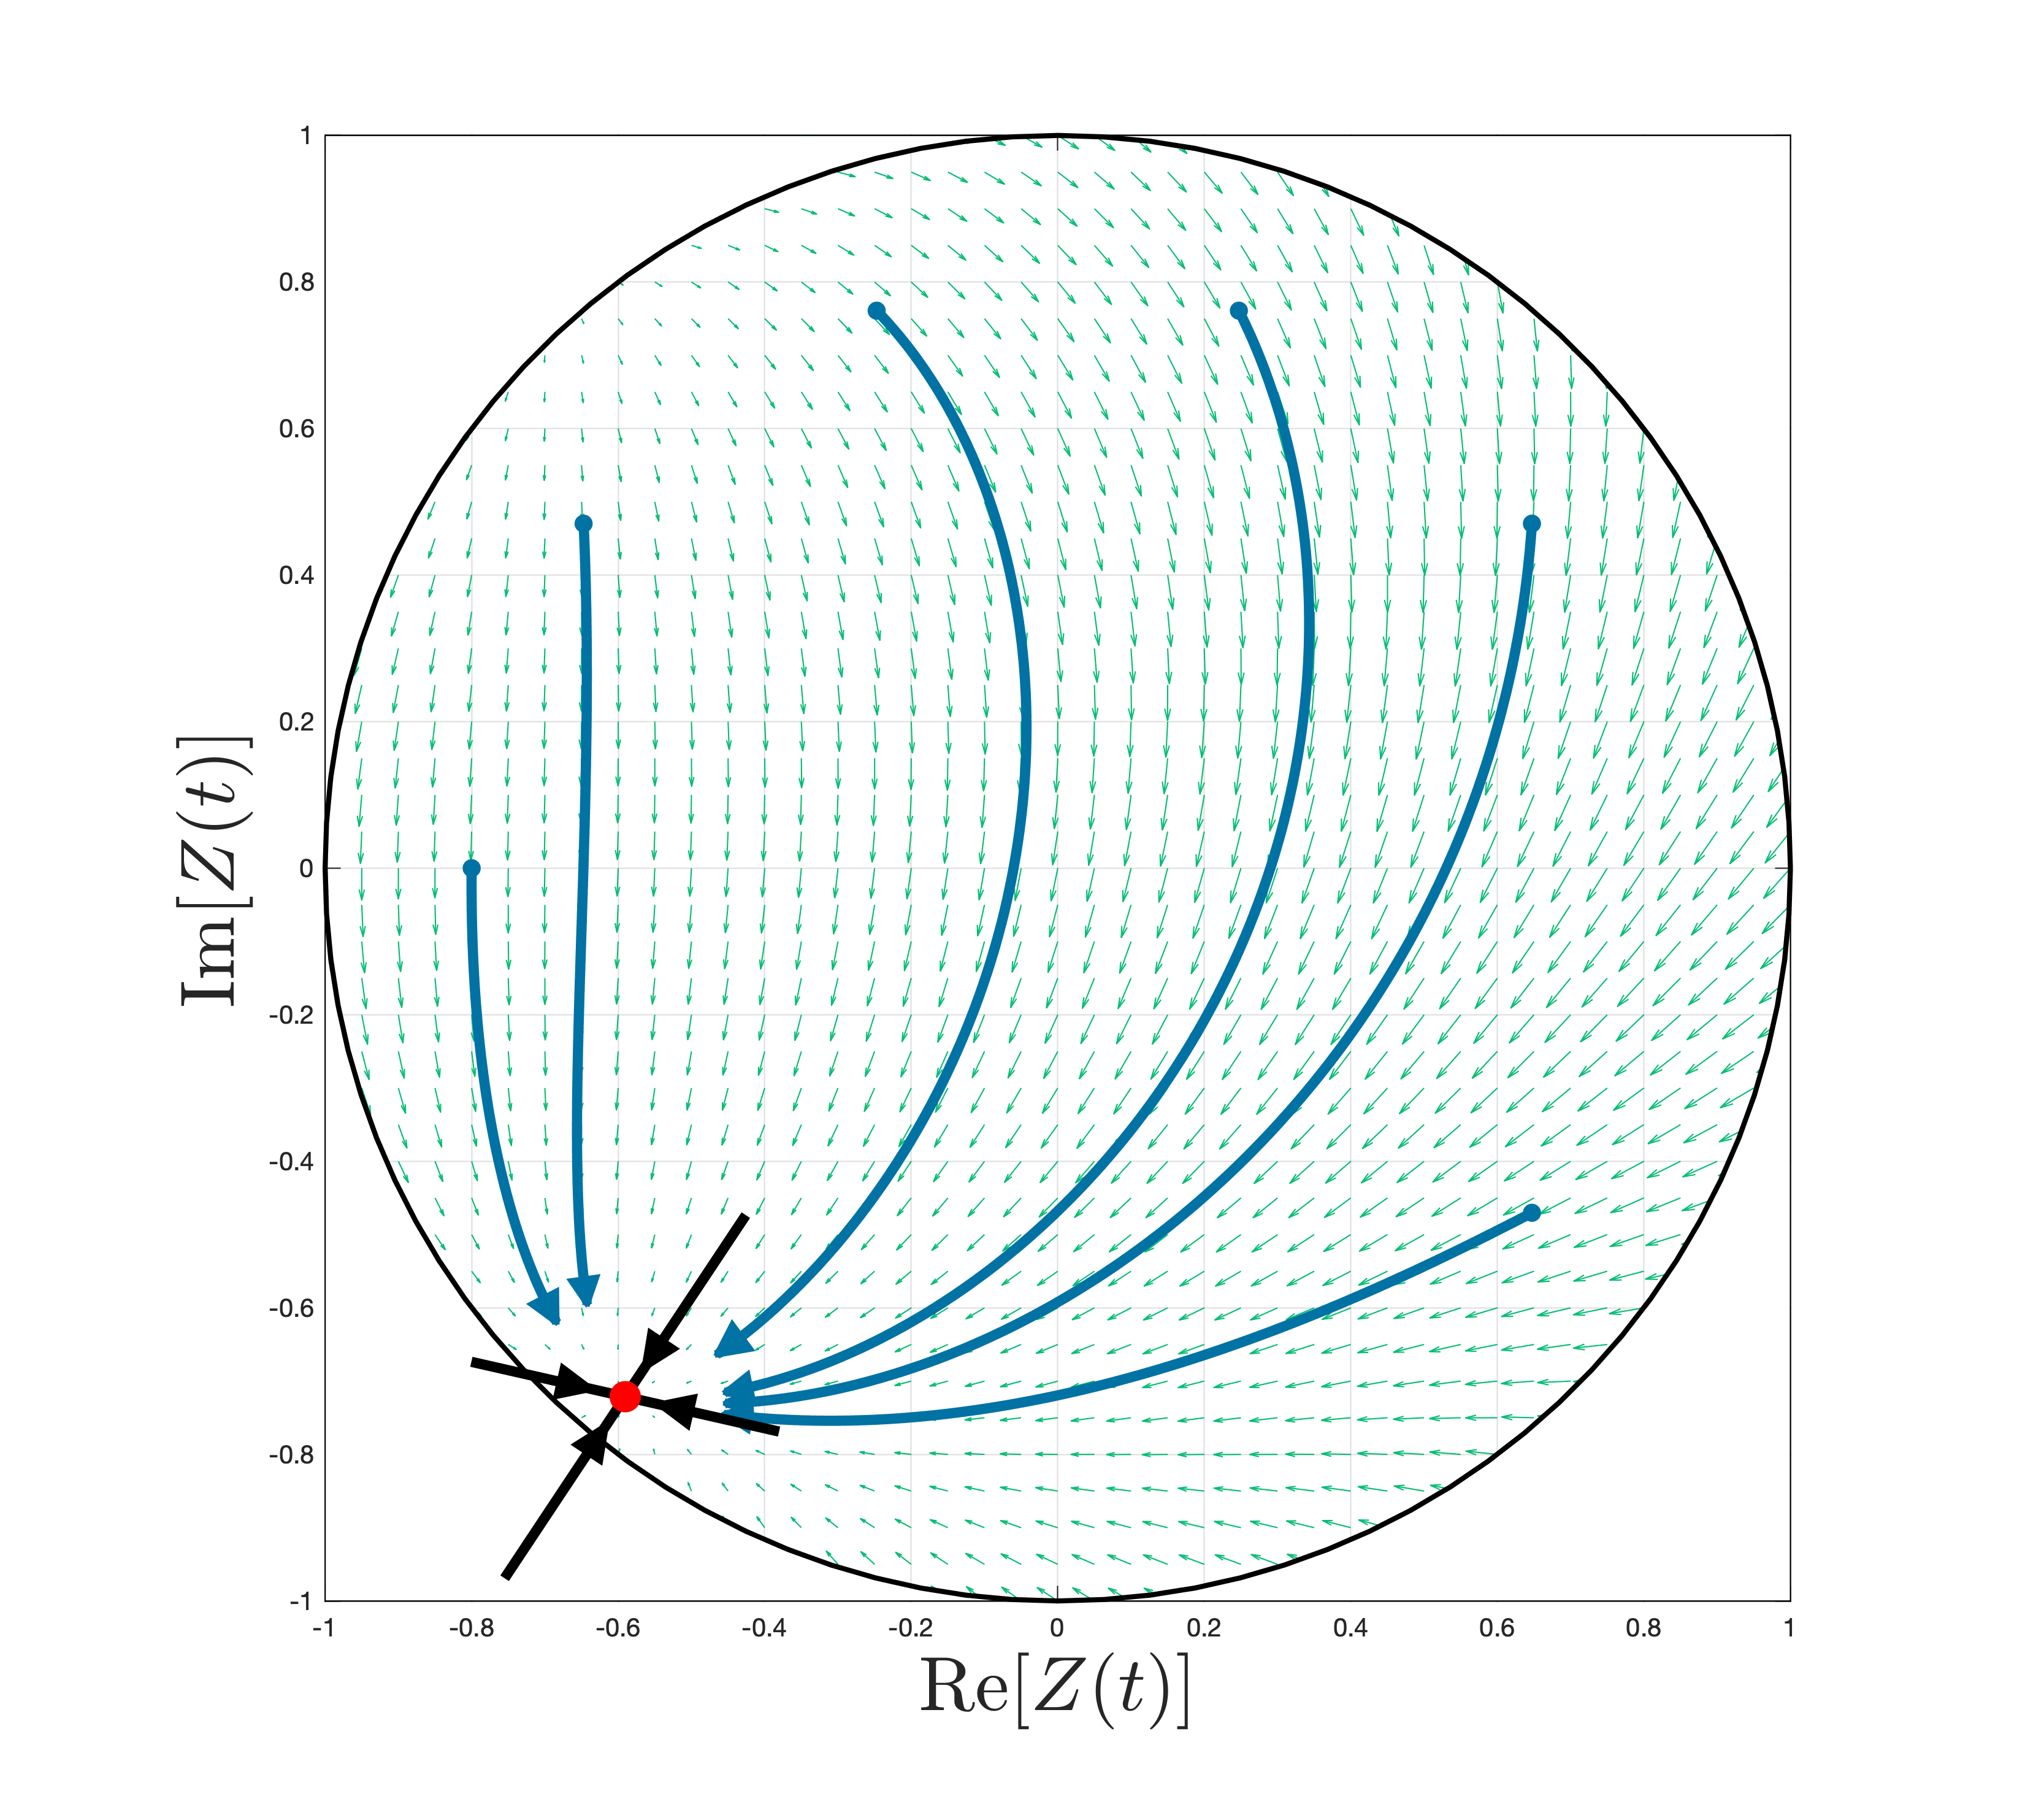
\includegraphics[width=\linewidth, trim={2cm 1cm 2cm 1.5cm },clip]{../Figures/PhaseSpace/MFRPSR.png}
   \caption{PSR state for $\eta_0 = -0.9, \sigma = 0.8$ and $\kappa= -2$. The mean field settles onto a stable node.}
   \label{fig:MFRPSR} 
\end{subfigure} \hfill
\begin{subfigure}[b]{0.32\linewidth}
   \centering
  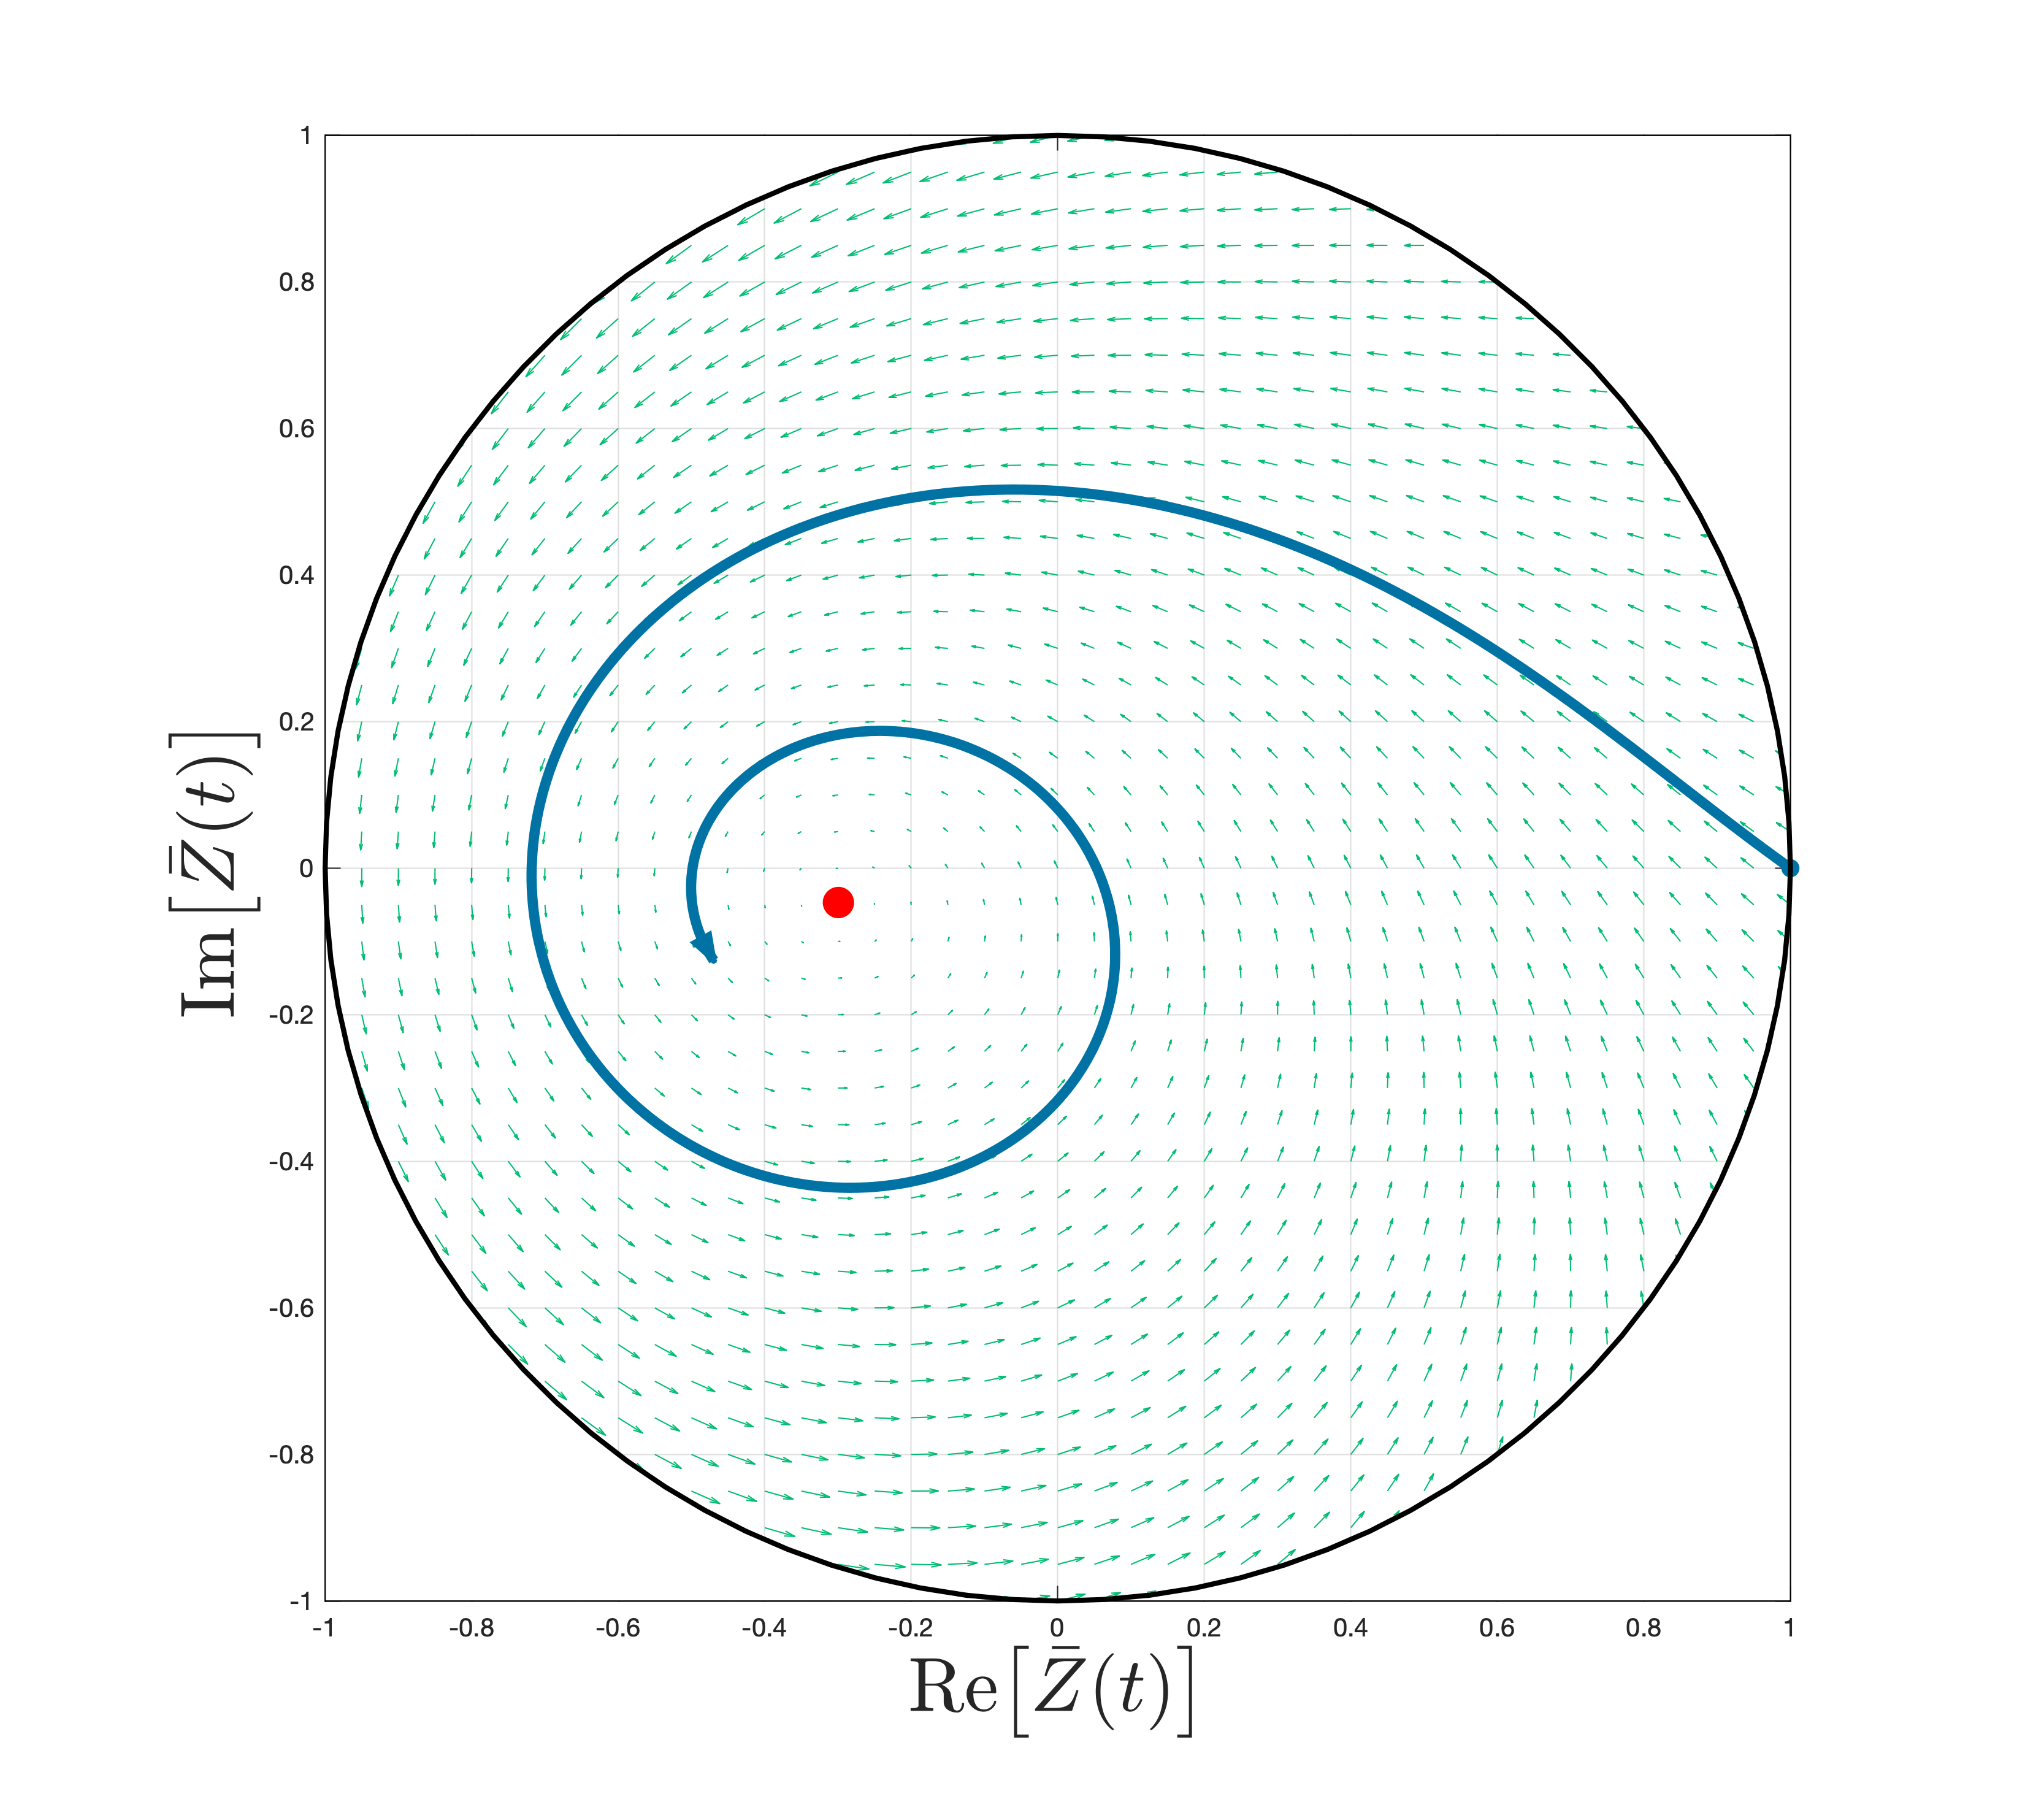
\includegraphics[width=\linewidth, trim={2cm 1cm 2cm 1.5cm },clip]{../Figures/PhaseSpace/MFRPSS.png}
   \caption{PSS state for $\eta_0 = 0.5, \sigma = 0.7$ and $\kappa= 2$. The mean field settles onto a stable focus.}
   \label{fig:MFRPSS}
\end{subfigure} \hfill
\begin{subfigure}[b]{0.32\linewidth}
   \centering
  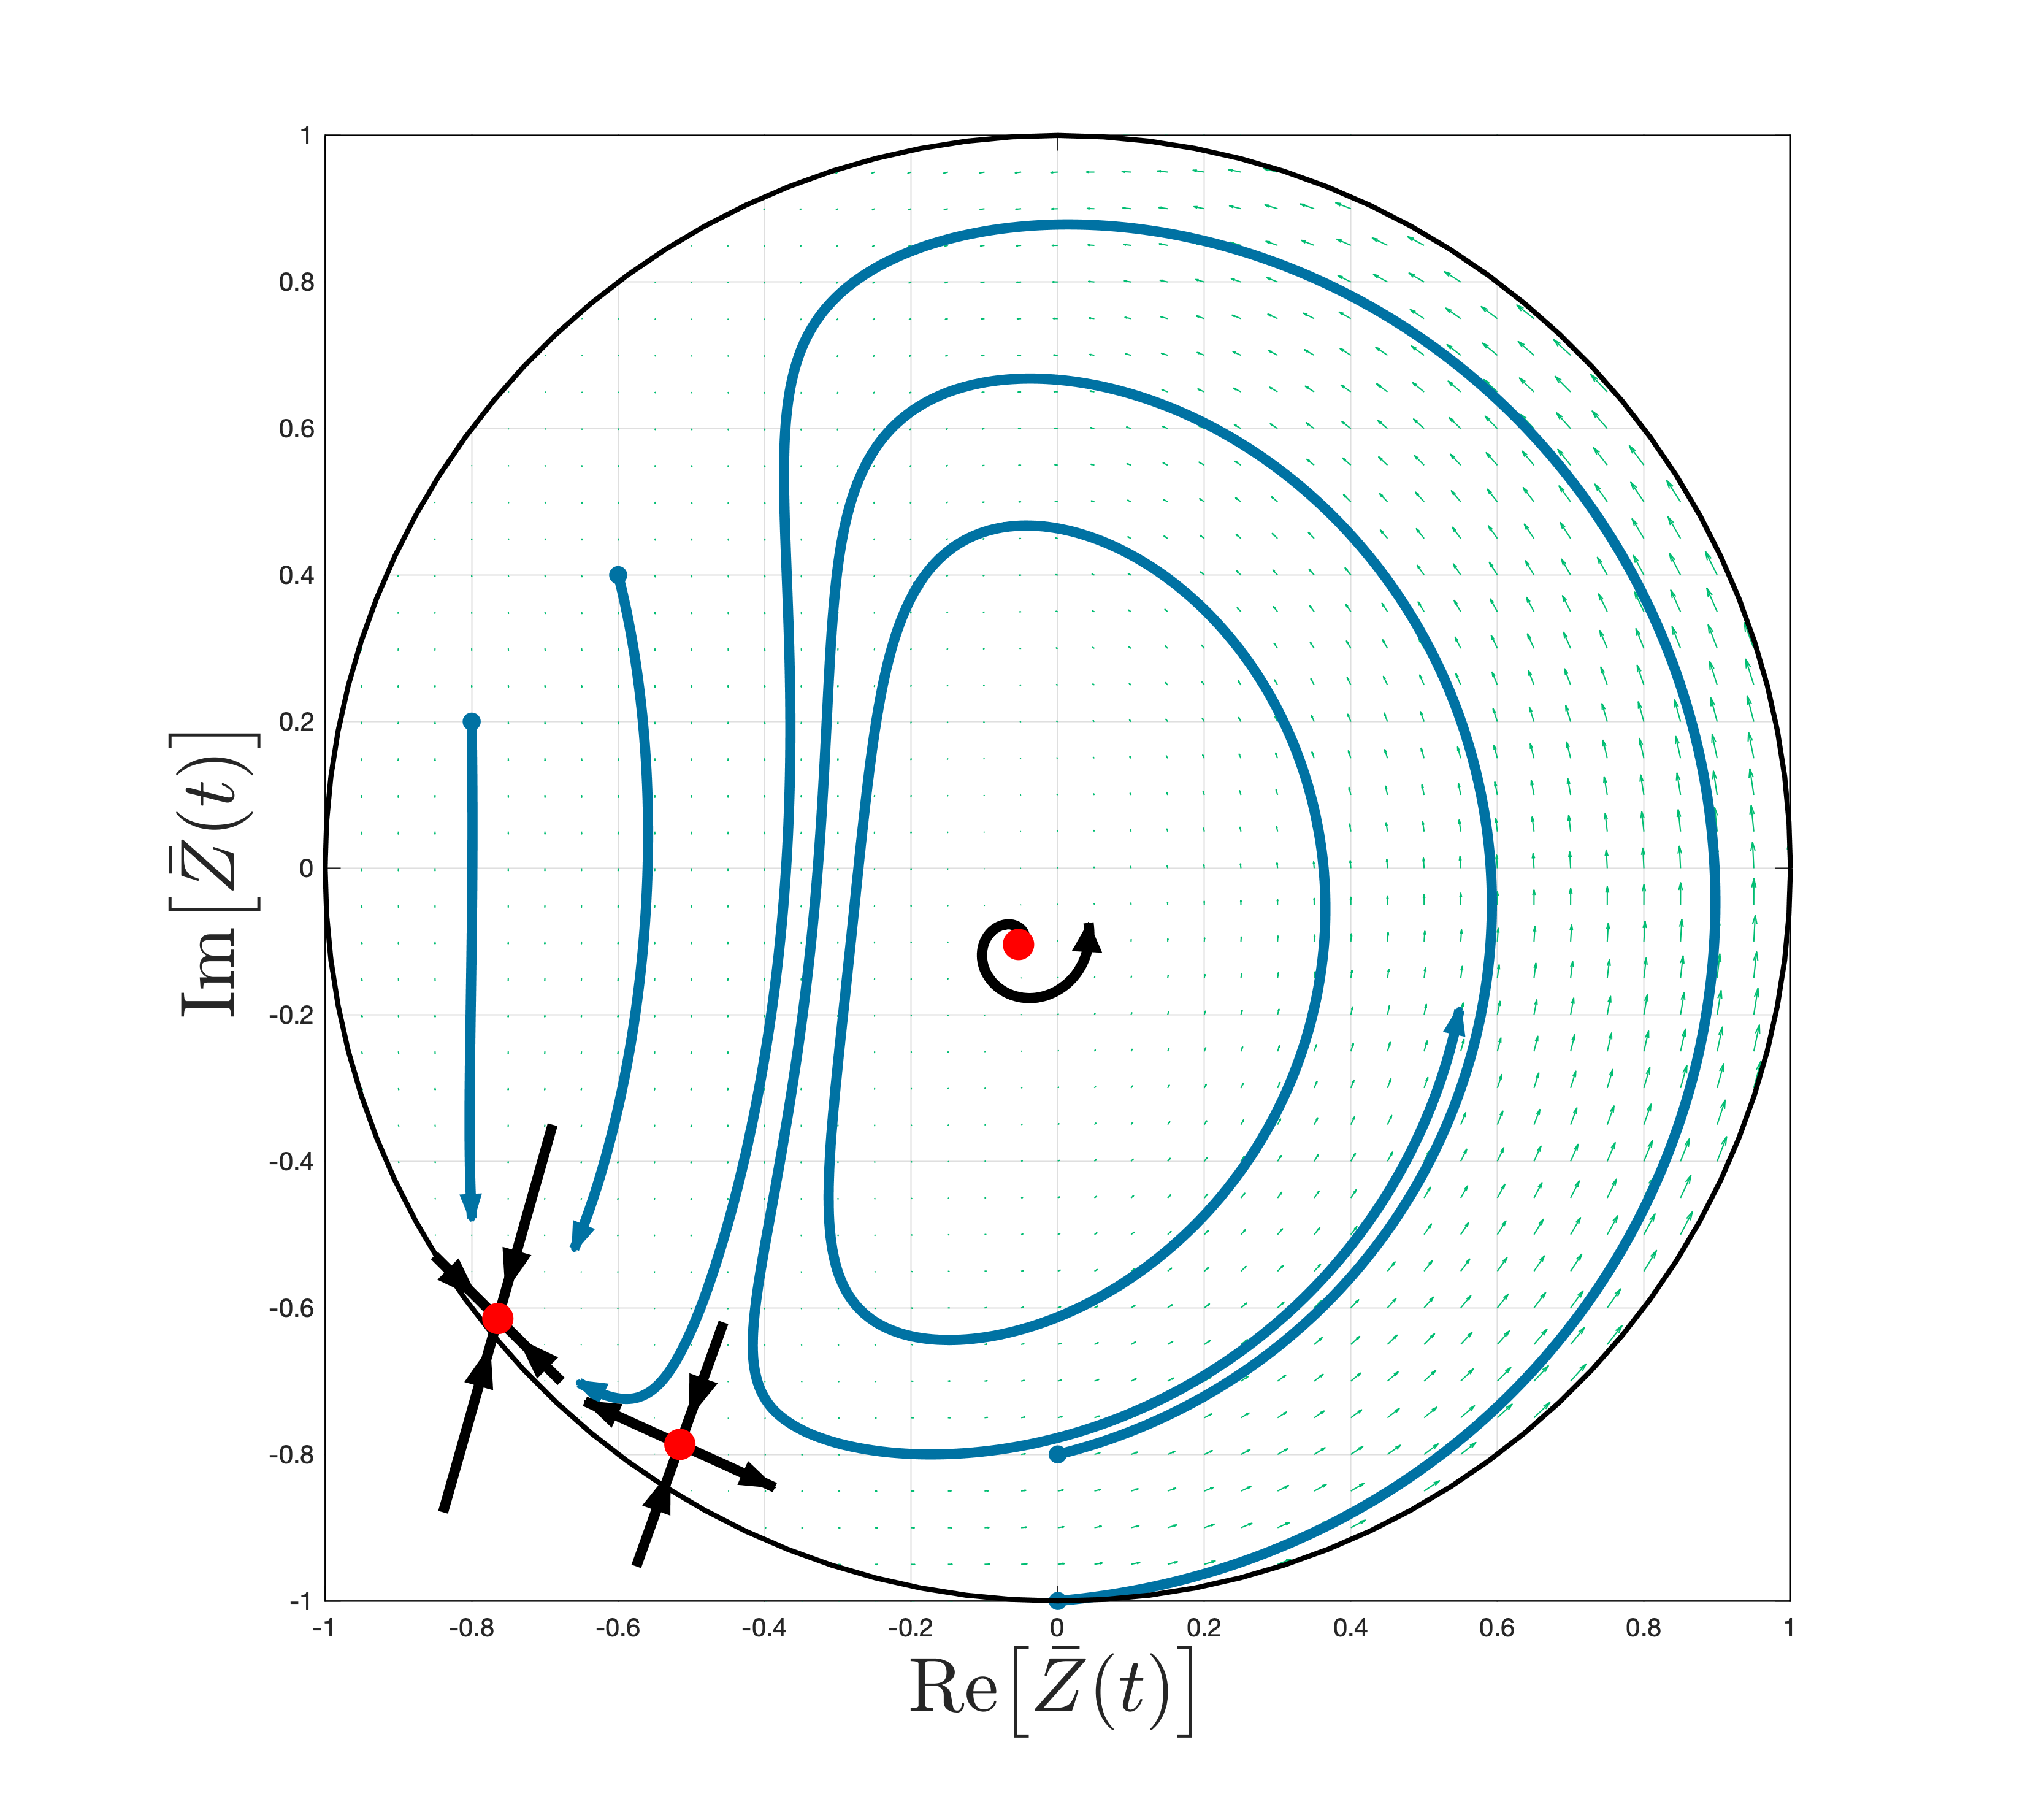
\includegraphics[width=\linewidth, trim={2cm 1cm 2cm 1.5cm },clip]{../Figures/PhaseSpace/MFRCPW.png}
   \caption{CPW state for $\eta_0 = 10.75, \sigma = 0.5$ and $\kappa= -9$. The mean field settles onto a stable limit cycle.}
   \label{fig:MFRCPW}
\end{subfigure}
   \caption{Three macroscopic states observed in the \MFR inside the imaginary unit circle $|Z(t)| = 1$. Green arrows mark the phase space vector field and blue trails mark solution curves. Red points indicate equilibrium points, with black arrows marking the direction of the eigenvectors in that point, scaled according to the magnitude of the corresponding eigenvalues.}
   \label{fig:macroscopicstatesfixeddegree}
\end{figure}



\subsection{The Ott-Antonsen extension to arbitrary network topologies}
In \cite{Restrepo2014} the authors extended their work to include networks with arbitrary degree distributions, applied to the Kuramoto model. An assortativity function was introduced to constrain the equations to respect a constant number of links in the network. Later this analysis was extended to networks of the Theta Neuron model \cite{OttAntonsen2017}. 

To simplify notation, the authors incorporate the network size in to $P$ so that $\sum_{\k \in \K} P(\k) = N$. The dynamics of the mean field are now given per degree in the network, that is to say: all nodes with the same degree $\k$ follow the same dynamics.
\begin{align}
\frac{\partial z(\k, t)}{\partial t} &= -\ic \frac{(z(\k, t)-1)^{2}}{2} + \frac{(z(\k, t)+1)^{2}}{2} \cdot I(\k, t) \qquad z(\k,t) \in \C^{M_\k} \nonumber \\
I(\k, t) &= -\sigma(\k) + \ic \eta_{0}(\k) + i H_2(\k,t) \label{eq:OttAntonsenSystemFull} \\
H_2(\k,t) &= \frac{\kappa}{\kmean} \sum_{\kacc \in \K} P\left(\kacc\right) a\left(\kacc \rightarrow \k\right) \cdot \left( 1 + \frac{z(\kacc, t)^2 + \overline{z}(\kacc, t)^2}{6} - \frac{4}{3} \Re(z(\kacc, t)) \right) \nonumber
\end{align}
This is the most general form of the theory, applied to our situation. In the following, we will allow independant variables $\eta_0 \equiv \eta_0(\k)$ and $\sigma \equiv \sigma(\k)$. $H$ is a legacy term that comes from the theory of the \MFR. $a$ is the assortativity function, which models the probability of a link from a node of degree $\kacc$ to one of degree $\k$:
\begin{align}
a\left(\kacc \rightarrow \k\right) = 0 \leq \frac{k_{\text{out}}^{\prime} k_{\text{in}}}{N \kmean} \leq 1 \label{eq:assortativityfunction}
\end{align}
where we have chosen a neutral assortativity \cite{OttAntonsen2017}. We can then find the mean field dynamics through:
\begin{align}
\overline{Z}(t) &= \frac{1}{N} \sum_{\k \in \K} P(\k) z(\k, t) \qquad \overline{Z}(t) \in \C \label{eq:OttAntonsenMeanField}
\end{align}

\eqref{eq:OttAntonsenSystemFull} yields an identical formulation as in \cite{Luke2013} and \cite{Martens2020} and for any fixed-degree network, it is a single complex differential equation. The \MFR is computationally efficient, and in \cite{OttAntonsen2017} many methods for improving this efficiency further are treated.

